\subsection{Parton Energy Loss and Jet Modification}
\label{Sec:Jets}

\subsubsection{Introduction}
\label{Sec:JetIntro}

In processes involving a hard scattering, highly virtual partons
are produced; these then undergo successive branchings resulting in a parton
shower~\cite{Field:1976ve}. The  ensemble of produced particles is highly collimated about
the direction of the initial parton and contains a range of different
momentum scales. The properties of these objects, known as jets~\cite{Sterman:1977wj}, and
how they emerge from perturbative QCD (pQCD) calculations have been extensively studied in high-energy
physics~\cite{Feynman:1978dt,Field:1977fa}. 




One of the successes of the early portion of the RHIC program
was the discovery of jet quenching\cite{Adcox:2001jp,Adler:2002xw}: the phenomenon in which jet showers are modified by interactions with the
medium~\cite{Bjorken:1982tu}. The most noticeable outcome of this scattering in the medium is an enhanced rate of bremsstrahlung leading to a 
loss of energy and momentum by the most energetic (leading) partons in the shower, which results in a depletion of high momentum hadrons. 
The first measurements of the suppression of high-\pT\ hadrons
and di-hadron correlations established that the medium was highly
opaque to colored probes. This indicated that the medium contains a
high density of unscreened color charges which lead to considerable modification of hard jets. 
Later measurements of single and dihadron observables at both RHIC and the LHC have significantly restricted
the variety of viable theoretical approaches to jet modification in a dense medium. 
%and that the final-state
%interactions induced by the medium result in the breakdown of usual
%pQCD factorization. 
%The high momentum constituents of the jets can be
%used to resolve the short distance structure and address whether
%quasi-particles are present in the medium. 


The virtuality of a hard parton within a jet represents its intrinsic scale, which is also the scale at which it resolves fluctuations in the medium. 
As partons in the jet cascade down to lower virtualities, they probe the medium over a multitude of length scales. 
As long as the virtuality (and the related resolution scale) of a parton is much larger than $\Lambda_{QCD}$, it will be weakly coupled to the medium and 
pQCD  describes its propagation, via both scattering and radiation in the medium.
The largest virtualities reside, on average, with the leading or highest energy parton, with lower energy partons decaying more rapidly to lower virtualities. 
It is this expectation that led to the formulation of the earlier pQCD based leading parton energy loss calculations~\cite{Gyulassy:1993hr,Wang:1991xy,Baier:1996kr,Baier:1996sk,Zakharov:1996fv,Zakharov:1997uu}. 
While scattering in the medium slows down the rate at which
the virtuality (and the related resolving power) decreases,
several partons within a jet still may lose sufficient amounts of energy and/or virtuality in the medium and encounter 
non-perturbatively strong coupling~\cite{Chesler:2008uy,Chesler:2008wd,Friess:2006aw,CasalderreySolana:2006rq}. 
While the fate of such partons is under some debate, the evolution of the leading hard partons with virtualities $Q^{2} \gg \Lambda_{QCD}^{2}$ has been successfully  
described using pQCD and factorized transport coefficients. This formalism and the experimental results related to it are described Section~\ref{q-hat-e-loss}. 

With the tremendous improvement in experimental abilities at the LHC, it has now become possible to reconstruct and isolate an entire jet from the dense fluctuating medium.
Experimental issues related to this development are described in Section~\ref{Sec:jet-reconstruct}. The modification of entire jets in a medium involves dynamical processes at energy scales 
ranging from the perturbative hard scale down to the non-perturbative soft scale of the medium. Recent empirical observations along with new theoretical insight dealing with phenomena at intermediate scales are discussed is 
subsection~(\ref{jet-mod}).
As jets provide probes at a
variety of scales, a program of systematic jet measurements can be
used to study the emergence of strongly-coupled behavior that has been
observed at long wavelengths in flow measurements, as well as its interplay with short distance fluctuations which affect the jet core. 
% through measurements sensitive to the near-perfect hydrodynamical evolution of
%the bulk medium.

\subsubsection{Leading hadron suppression and jet transport coefficients}~\label{q-hat-e-loss}

%After more than a decade of RHIC running and including the results of the LHC heavy-ion experiments, a \emph{standard model} of heavy-ion collisions has emerged:  Phenomena at the 
%\emph{softest} scales in the collision are explained by \emph{viscous fluid dynamics}, while those at the \emph{hardest} scales have been demonstrated to be describable by \emph{weakly coupled perturbative QCD}. 
At the time of this writing, jets have been measured at the LHC with energies up to several hundred GeV, while jets at RHIC have been measured with energies up to 50 GeV.
These exhibit non-trivial interaction with the medium over a wide range of scales.  
The collimated shower of partons contain a central, \emph{hard core} that consists of the leading partons, which carry a majority of the jet's momentum.
These partons are the dominant contributors to leading hadron analyses such as the single hadron inclusive nuclear modification factor, or leading hadron triggered near and away side correlations. 
Calculations that focus solely on this hard core~\cite{Gyulassy:2000er,Arnold:2002ja,Qin:2007rn,Wang:2001ifa,Majumder:2009ge,Majumder:2011uk} 
have been quite successful at describing several of these single particle observables. 
%r, both integrated and as a function of the reaction plane,


When produced in vacuum, jets tend to shower to several partons with progressively lower virtualities. 
In the case where the jet is produced in a medium, those partons in the jet with 
virtualities that considerably exceed $\Lambda_{QCD}$ are weakly coupled to the medium. Therefore, the 
radiation from and scattering of these partons are calculable in pQCD. 
The scatterings induce shifts both in the momentum of the propagating partons and in their virtuality. As a result, these scatterings change the radiation pattern of the shower by inducing longitudinal drag (and associated longitudinal diffusion), transverse diffusion, and enhanced splitting of the propagating partons. The transport coefficients 
$\hat{q}$~\cite{Baier:2002tc} and $\hat{e}$~\cite{Majumder:2008zg} quantify the transverse diffusion and longitudinal drag experienced by a single hard parton, and are the leading transport coefficients that modify the propagation and in-medium splitting of hard jets. 


The transport coefficient $\hat{q}$ characterizes the mean-squared momentum per unit length acquired by a parton transversing the medium.
Formally, it is the Fourier transform of the Lorentz-force-Lorentz-force correlator, 
which for a near on-shell parton traveling in the negative light cone direction with momentum $q^{-}$ in a gauge with $A^{-}=0$ gauge is
\begin{eqnarray}
\hat{q} (x^{-}) = \frac{8\pi^{2} \alpha_{S} C_{R}}{ N_{c}^{2} - 1} \int \frac{d^{2} y_{\perp} dy^{-} d^{2} k_{\perp} }{(2 \pi)^{3}} e^{-i \frac{k_{\perp}^{2} }{2q^{-}} y^{-} + i \vec{k}_{\perp} \cdot \vec{y}_{\perp} }  \langle F^{+ \mu}  (x^{-} + y^{-}, \vec{y}_{\perp}) F^{+}_{\mu}(x^{-},0) \rangle.
\label{Eq:qhat}
\end{eqnarray}
%
In this expression, $\langle \cdots \rangle$ implies an expectation over the state (or states) of the medium. The field strength tensor $F^{\mu +} \equiv F^{a \mu +} t^{a}$ represents 
the soft color field of the medium off which the hard parton with color Casimir $C_{R}$ scatters (trace over color indices is implied). 
%Wide ranging studies of such observables, including more differential reaction plane dependent measurements, as well as full-jet measurements at the LHC (and RHIC), have established the picture in which these leading hard partons in the jet shower undergo multiple scattering in the dense medium, resulting in an enhanced rate for radiating partons with a softer momentum profile than in vacuum. While the entirety of these showers, in particular, the softer partons at lower invariant off-shell mass cannot be expected to be weakly interacting with the medium, the modification of the harder partons has been successfully described in terms of jet transport coefficients. These are factorized from the hard dynamics of parton splitting, and encode the effect of the soft medium on a parton, e.g., in terms of its transverse momentum diffusion rate $\hat{q}$, the longitudinal momentum drag rate $\hat{e}$ etc. 
These soft matrix elements are 
factorized from the hard processes of parton propagation and splitting~\cite{Kang:2013raa}. In simplified scenarios, such as in a static thermal medium, 
they may be calculated from first principles assuming that the medium is 
weakly coupled~\cite{CaronHuot:2008ni}, strongly coupled~\cite{Liu:2006ug}, on the lattice~\cite{Majumder:2012sh}, or using a combination of weak coupling and 
lattice techniques~\cite{Panero:2013pla}. However, for the dynamical rapidly expanding medium created in relativistic heavy ion collisions, the only recourse is to extract averaged soft matrix elements by comparing experimental results to calculations that involve 
detailed treatments of hard parton production, shadowing, and final state parton propagation in media simulated with viscous fluid dynamics. 
In such calculations, $\hat{q}$ is either recalculated assuming a weakly coupled medium once the coupling constant in the medium is fit to data (as in Ref.~\cite{Gyulassy:2000er,Arnold:2002ja,Qin:2007rn}), or it is scaled with an intrinsic quantity in the hydrodynamic simulation, with the overall normalization fit to data (as in Ref.~\cite{Majumder:2011uk}).  

\begin{figure}[t]
\centerline{
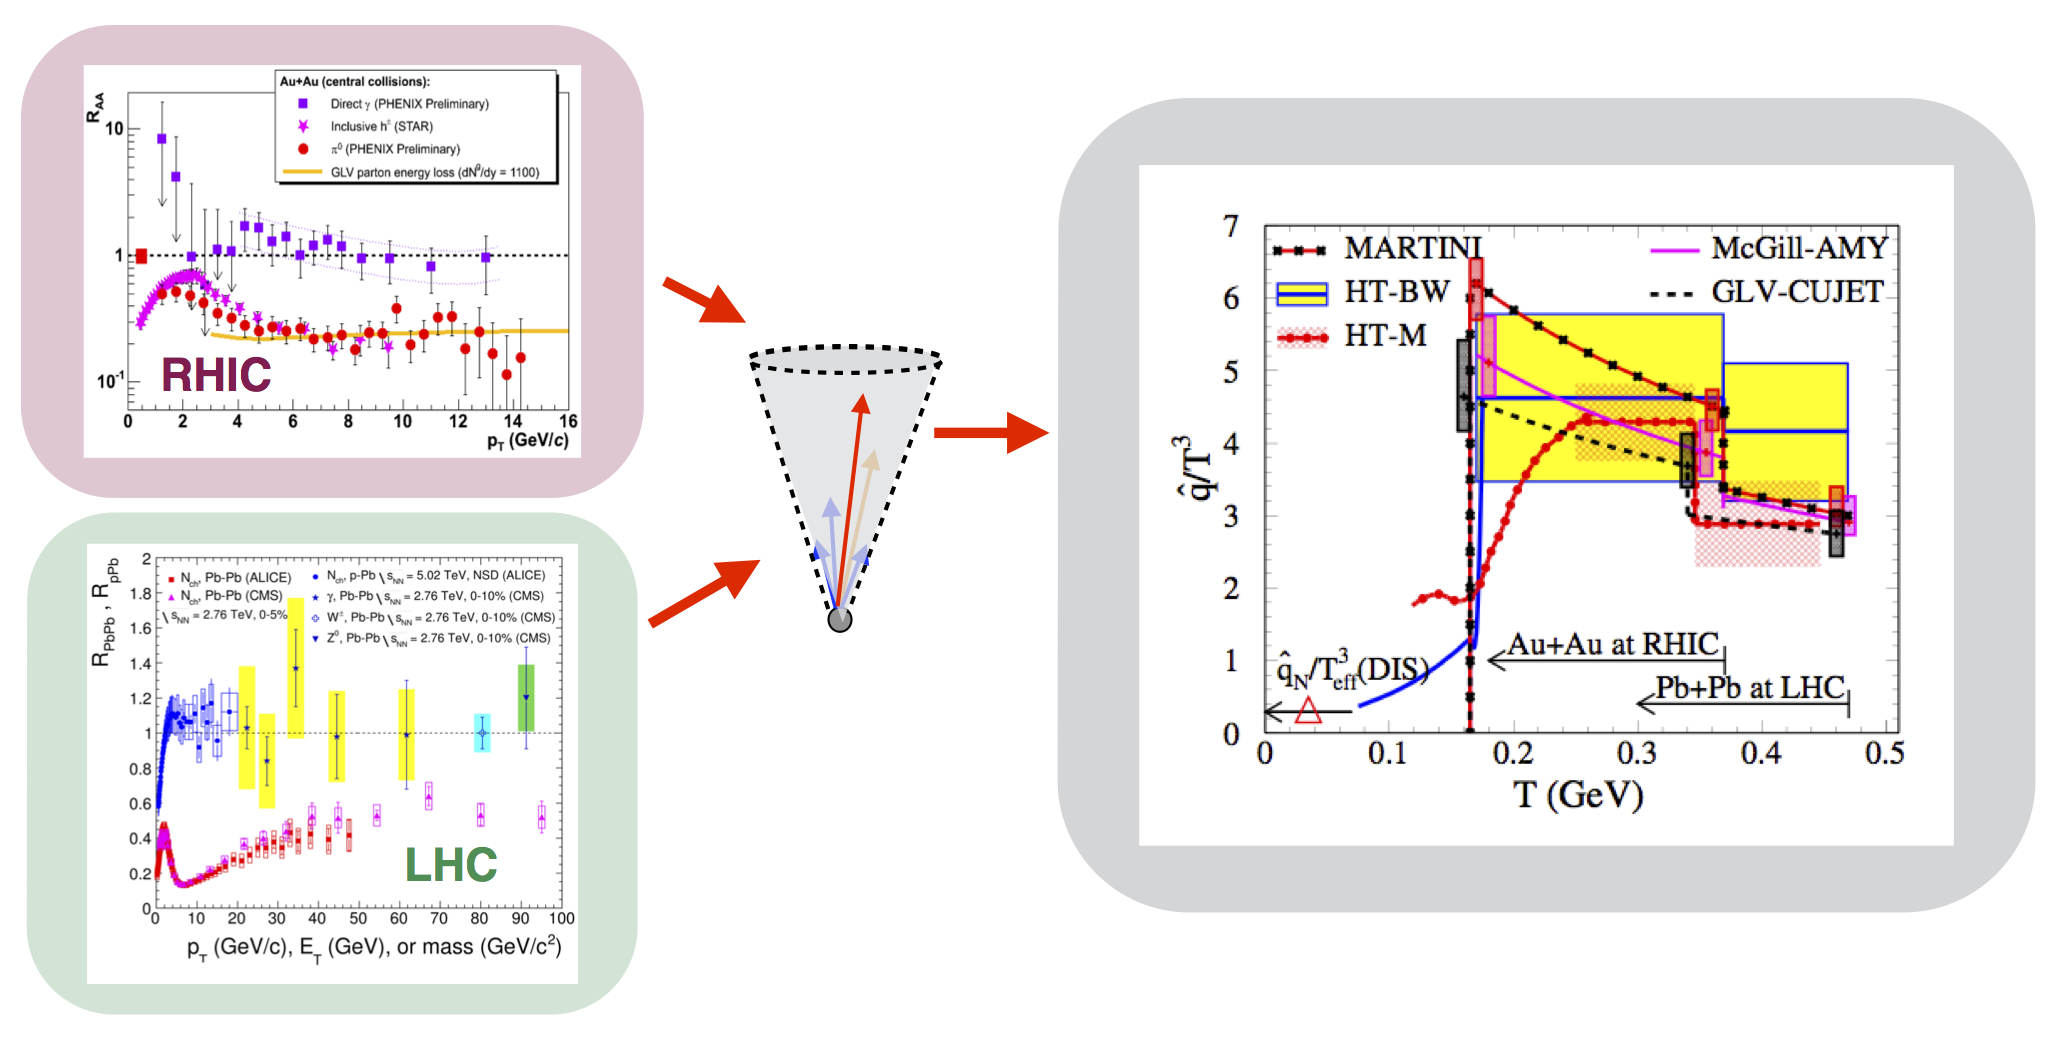
\includegraphics[width=1.03\textwidth]{fig/JetProgressFig1_v2}}
\caption[RHIC and LHC data compared to different pQCD energy loss energy loss schemes]{A comparison of several different pQCD based energy loss energy loss schemes to the measured leading hadron suppression in central events at RHIC and the LHC, and the extracted transport coefficient $\hat{q}$ along with its dependence on temperature.}
\label{fig:JetProgressFig1}
\end{figure}


In either of these approaches, one obtains a very good description of the experimental results on the suppression of leading hadrons from both RHIC and the LHC. Some of these fits are shown in the left panel of Figure~\ref{fig:JetProgressFig1}.
The extracted values of the leading transport parameter $\hat{q}$ and its temperature dependence are plotted in the right panel of Figure~\ref{fig:JetProgressFig1}. Using identical 
initial states and hydro simulations, 
the JET Collaboration\footnote{The JET Collaboration is one of the Topical Collaborations in nuclear theory established by the DOE Office of Nuclear Physics in response to a recommendation in the 2007 Long-Range Plan for Nuclear Physics.}\cite{JET}
has carried out the analyses of comparing the spread in values of $\hat{q}$ due to systematic differences in the pQCD based 
energy loss schemes~\cite{Burke:2013yra}. In sharp contrast to similar comparisons carried out earlier in Ref.~\cite{Bass:2008rv}, where extracted  $\hat{q}$ values differed by almost an order of magnitude, current calculations reported in Ref.~\cite{Burke:2013yra}, differ at most by a factor of 2, 
indicating the very considerable progress in our understanding of hard processes in the QGP since the time of the last Long Range Plan.

Beyond the success of applying pQCD based energy loss techniques to the in-medium modification of leading partons in a hard jet, 
this five-fold reduction in the uncertainty of the 
extracted values of transport coefficients is greatly significant, as it allows, for the first time, 
to discern a possible non-monotonic dependence of $\hat{q}$ on the temperature of the medium. Hence, such theoretical analyses have reached a level of 
sophistication where qualitative and quantitative properties of the QGP may be extracted, with quantified systematic uncertainties, using jet modification. 
%
%Recent studies using a variety of different approaches to pQCD based jet modification, systematically conducted with identical initial state and soft medium simulations, have isolated the normalization of the leading transport coefficient $\hat{q}$ and also demonstrated the possibility of a non-trivial temperature dependence near the cross over transition. This represents both a qualitative and a near 5 fold quantitative improvement in our understanding of the hard dynamics of leading partons in a jet, propagating through a dense medium. 
These successes, enabled by improvements on the theoretical and experimental side, provide an anchor in our study of the modification of full jets in a medium, which involves an interplay of several different scales, as one moves from leading partons to the softer segments of the jet and their interaction with the medium. The incorporation of such theoretical improvements, and the ensuing measurements 
over the next decade
will allow jets to be used as calibrated and controlled precision probes of the microscopic structure of the quark-gluon plasma over a wide range of scales.


\subsubsection{Full jet reconstruction}
\label{Sec:jet-reconstruct}
Fully reconstructed jets have been a crucial tool used in high energy
physics, both to provide precision tests of pQCD and to understand the
topology of the hard-scattering event. Recently these techniques have
been adapted to the heavy ion environment resulting in a new set of
observables sensitive to jet quenching. Reconstructed jets are
expected to be related to initial parton kinematics and thus manifest
the kinematics of the hard scattering in the absence of medium
effects. Some of the first LHC heavy-ion results included the
observation of highly asymmetric dijet events, which provided a
striking visual demonstration of the energy
loss\cite{Aad:2010bu,Chatrchyan:2011sx}. Since these initial
measurements experimental control over the measured jet energies and
the understanding of the role of underlying event fluctuations has
improved substantially, resulting in precise measurements of jet
suppression and the properties of quenched jets. Color-neutral objects
such as a photons are not expected to experience quenching, and
measurements of direct photon production rates at
RHIC\cite{Adler:2005ig} were important in the interpretation of the
high-\pT\ hadron suppression. Recently, these measurements have been
extended to much higher \pT\
\cite{Aamodt:2010jd,Abelev:2012hxa,CMS:2012aa}, and additional probes
such as the $W$ and $Z$ \cite{Chatrchyan:2012nt,Aad:2013sla,
Chatrchyan:2011ua,Aad:2012ew} are accessible at the LHC. In events
where these objects recoil against a jet, they serve as relatively
clean probes of the jet kinematics before energy loss. The first
photon-jet measurements at the LHC \cite{Chatrchyan:2012vq} have shown
that the energy of these jets is significantly degraded and that in
many cases no recoil jet is distinguishable from the bulk medium.

\begin{figure}[t]
\centerline{
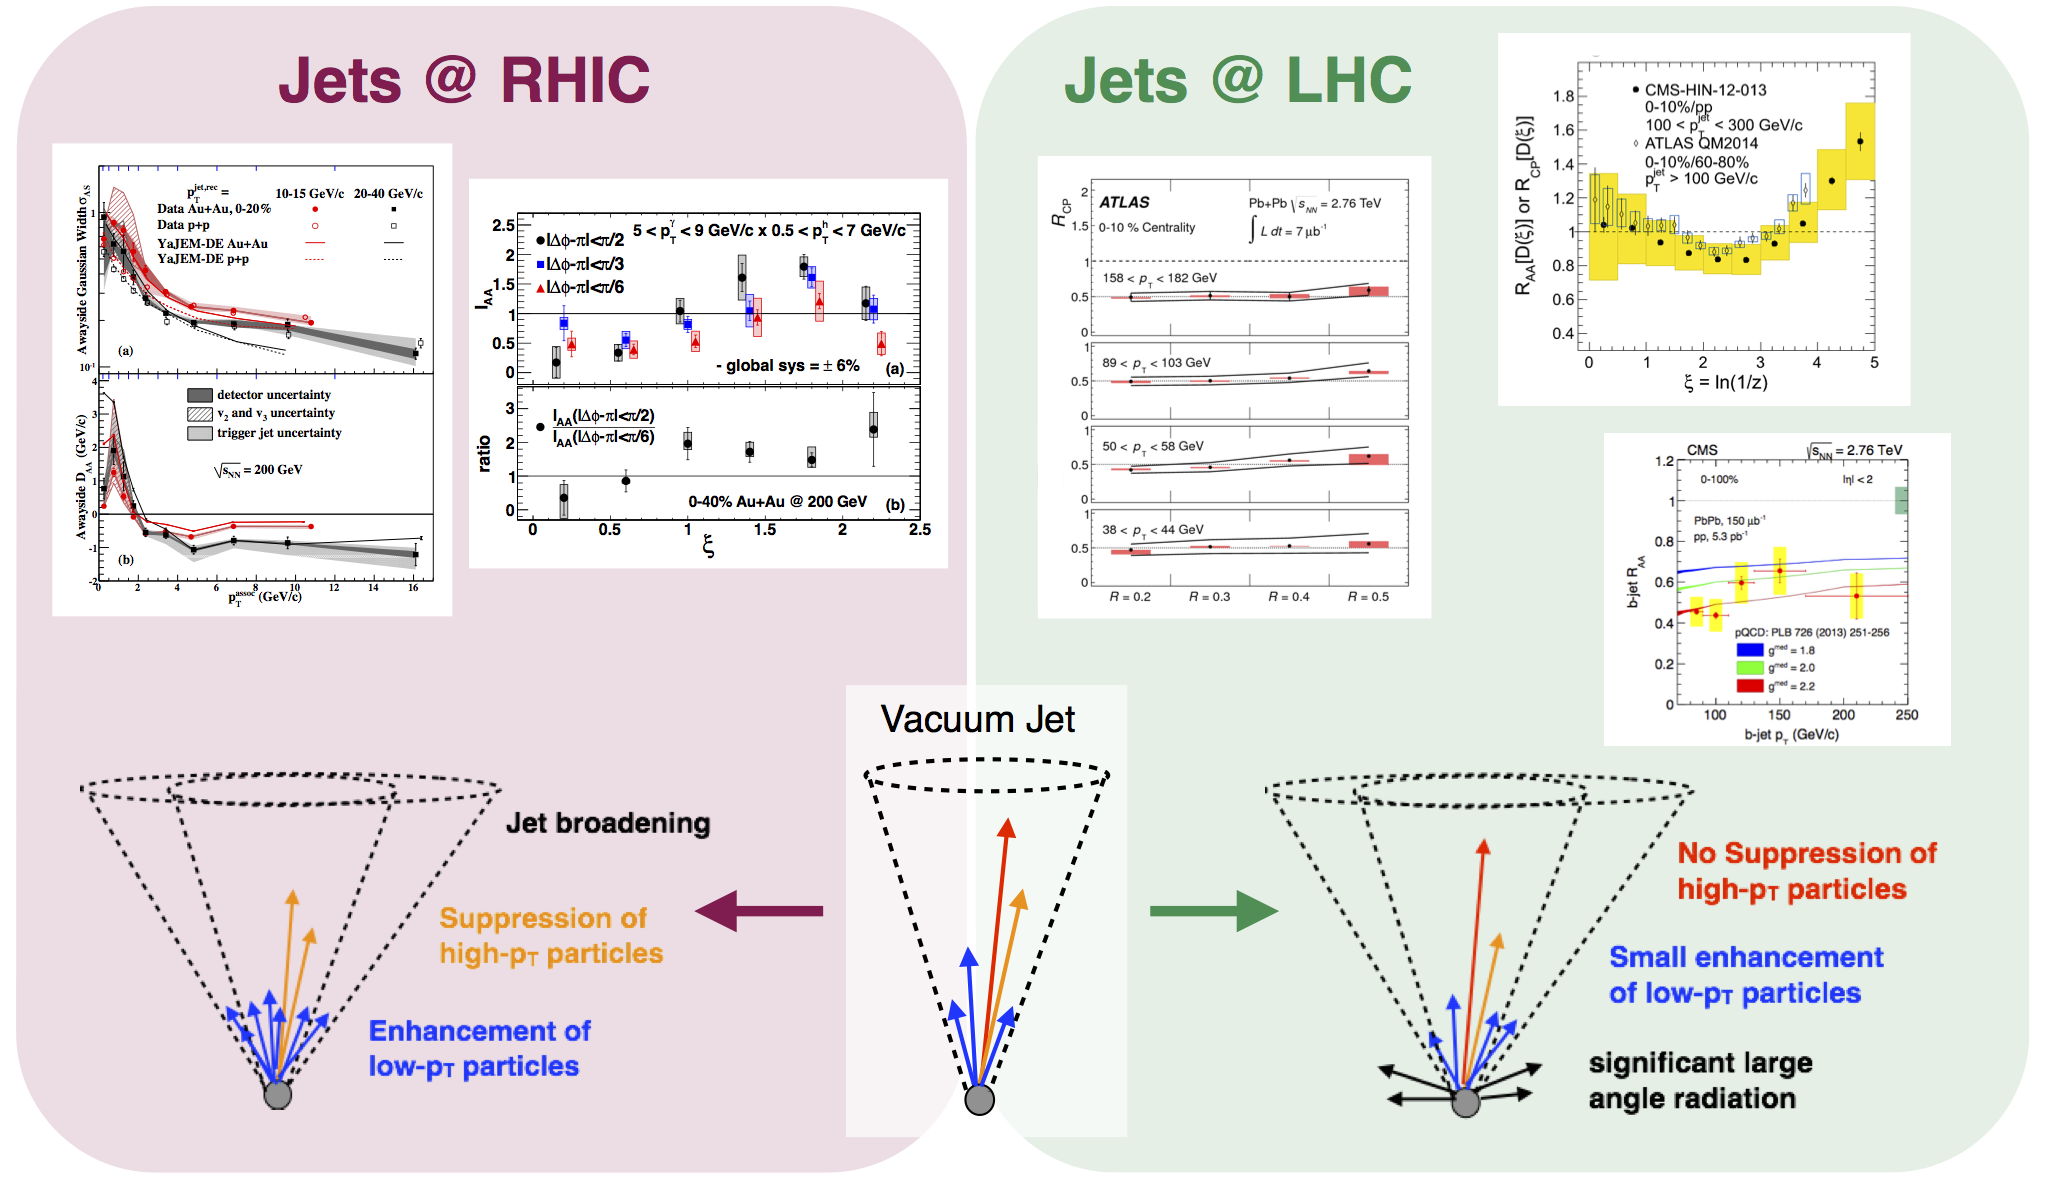
\includegraphics[width=0.99\textwidth]{fig/JetProgressFig2_v2}}
\caption[Qualitative summary of current jet/photon-hadron correlation measurements]{Qualitative summary of current jet/photon-hadron correlation measurements at RHIC (left panel) and selected full jet, $b$-jet $R_{AA}$ and jet fragmentation function measurements at the LHC (right panel). }
\label{fig:JetProgressFig2}
\end{figure}


\subsubsection{Jet modifications by the medium}~\label{jet-mod}
  
  While the experiments at RHIC have discovered that the medium created in heavy-ion collisions is opaque to energetic partons and initiated ground breaking attempts to measure the parton energy loss with jets, it was at the LHC where experimentalists have been able to leverage high kinematic reach of the collisions and unambiguously provide the evidence for jet momentum modifications. Utilizing the inclusive rates of high-energy jets and the momentum balance of back-to-back jets, photon-jet and hadron-jet coincidences, well described by pQCD in elementary/pp collisions, the experimental findings at the LHC strongly advanced the understanding of the depletion of the energetic jets in heavy-ion collisions. From these measurements two fundamental properties of jet-medium interactions have been established:
  \begin{itemize}
  \item the energy that is deposited into the medium is not recovered/contained within the jet cone as the rates of high-energy fully reconstructed jets in heavy-ion collisions are much less (about a factor of two) as compared to the expectation from proton-proton collisions (Figure\ \ref{fig:JetProgressFig2}, right panel);
  \item the interaction with the medium does not alter the direction of the propagating jet: although the distribution of the di-jet energy balance is strongly modified there is no sign of medium induced accoplanarity of the jet pairs.
  \end{itemize}
  Moreover, studies of the internal jet structure revealed that the recoiling jets that are 
%predestined by the construction of the analyses 
selected to lose a significant portion of their energy on average show moderate or only small modifications of their fragmentation pattern as compared to jets fragmenting in vacuum (Figure\ \ref{fig:JetProgressFig2}, right panel). On the other hand, the subsequent search for the radiated energy has provided evidence that it is redistributed over large angles away from the jet axis and hadronizes into soft (of the order of GeV) particles. In contrast, measurements utilizing jet/photon-hadron correlations at RHIC indicate that (on average) the fragmentation pattern is suppressed at high \pT\ and significantly enhanced at low \pT\ accompanied by only a moderate broadening of the jet structure (Figure\ \ref{fig:JetProgressFig2}, left panel). 
There now exist several model studies~\cite{CasalderreySolana:2011rq,Qin:2010mn} as well as a Monte-Carlo study~\cite{Perez-Ramos:2014mna} based on pQCD which demonstrate similar effects. It should also be pointed out that, at a qualitative level, such observations are not inconsistent with expectations for how jets
should lose energy in a strongly coupled plasma that are based upon
calculations done in model systems that can be analyzed using holographic duality.
Reconciling these findings in a coherent and quantitative theoretical parton energy loss framework will ultimately require from the experimental side a suite of similar jet measurements at RHIC to allow a direct comparison to LHC results.
  %{ \it Speculation: Investigations of the momentum dependence of the di-jet and photon-jet coincidences provided a phenomenological estimates that jets loose of the order of 15 GeV on average.} 
  
\subsubsection{Heavy quark energy loss}

Heavy quarks (in particular $b$ and $c$ quarks) provide both a systematic test of the underlying formalism of energy loss as well as access to a slightly different set of transport coefficients in the medium. As such they constitute a vital addition to the suite of jet observables. It should be made clear that here we refer to intermediate energy heavy quarks, i.e., quarks with a momentum $p$ relative to the medium satisfying $p \gtrsim M_{B}$, where $M_{B}$ is the mass of the bottom quark. 
Heavy quarks that have a lower momentum interact strongly  with the medium and will be covered in Section~\ref{Sec:HF}, while
quarks with momenta that are orders of magnitude larger than the mass can be treated as light quarks. It is in this intermediate momentum region where a considerable suppression in the yield of heavy quarks has been observed, either via the nuclear modification factor of non-photonic electrons at RHIC or via the nuclear modification factors of heavy flavor mesons at the LHC. At high momentum one expects heavy quark energy loss to be similar to that of light flavors. 


The extra and unexpected suppression at intermediate momenta has been the subject of intense theoretical work over the last several years. In Figure~\ref{Fig:non-photonic-suppression}, we show the 
experimental measurements for the nuclear modification factor for non-photonic electrons (the data are identical in all three plots). 
These measurements are compared with theoretical calculations from the ASW~\cite{Armesto:2003jh}, 
Higher-Twist~\cite{Qin:2009gw}, and WHDG~\cite{Wicks:2005gt} schemes. Both the WHDG and Higher-Twist calculations contain drag loss in addition to radiative loss and fit the data much better than the ASW curve which 
only contains radiative loss. 

%\begin{figure}[t]
%$\mbox{}$
%\!\!\!\!\!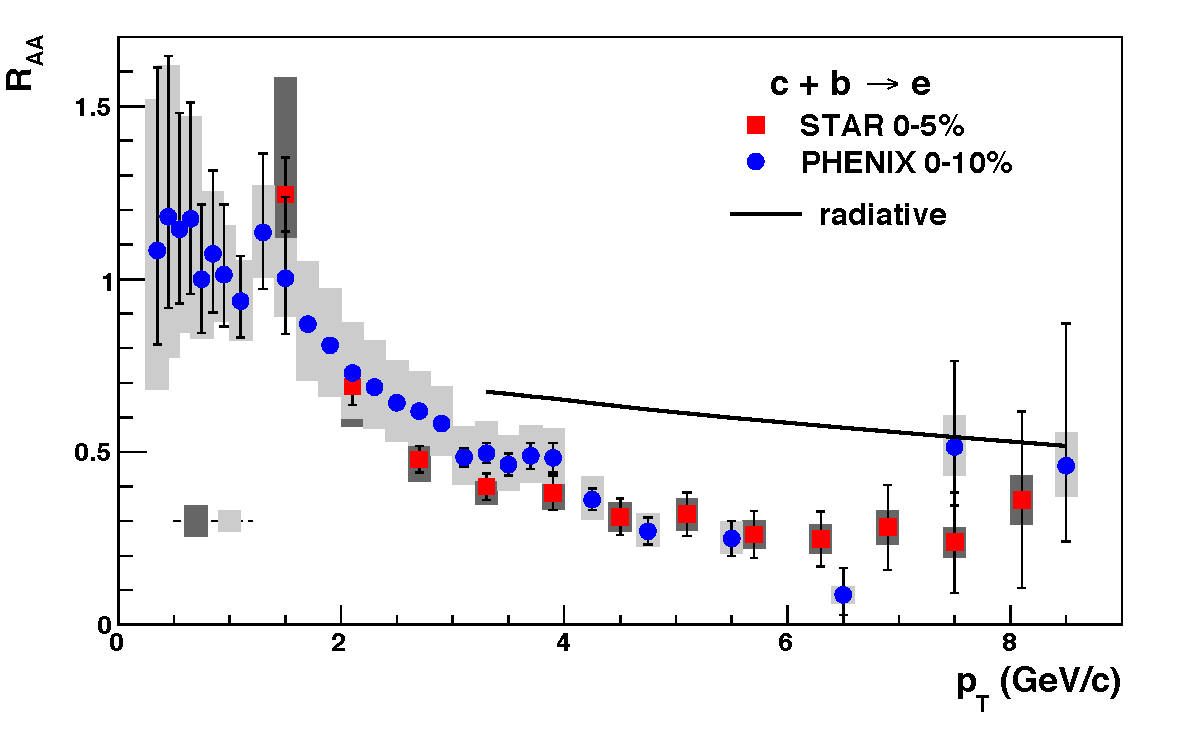
\includegraphics[width=0.35\textwidth]{fig/raa-nonphot-armesto}\!\!\!\!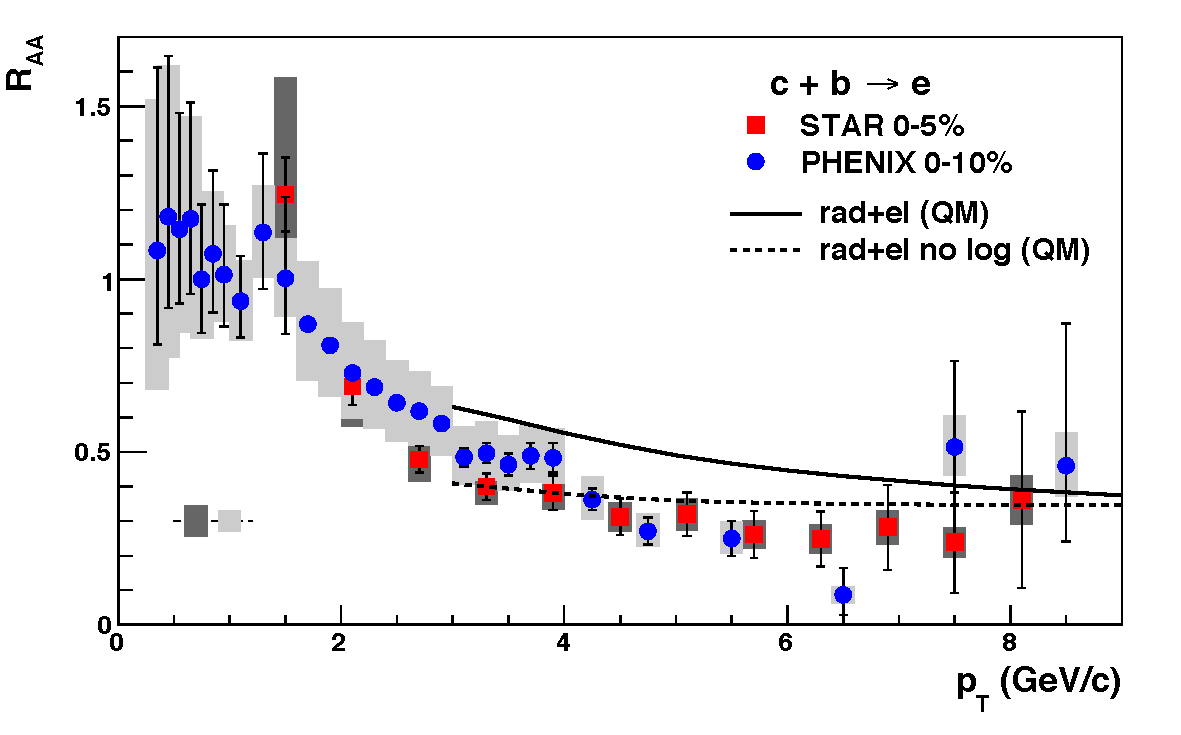
\includegraphics[width=0.35\textwidth]{fig/raa-nonphot-qin}\!\!\!\!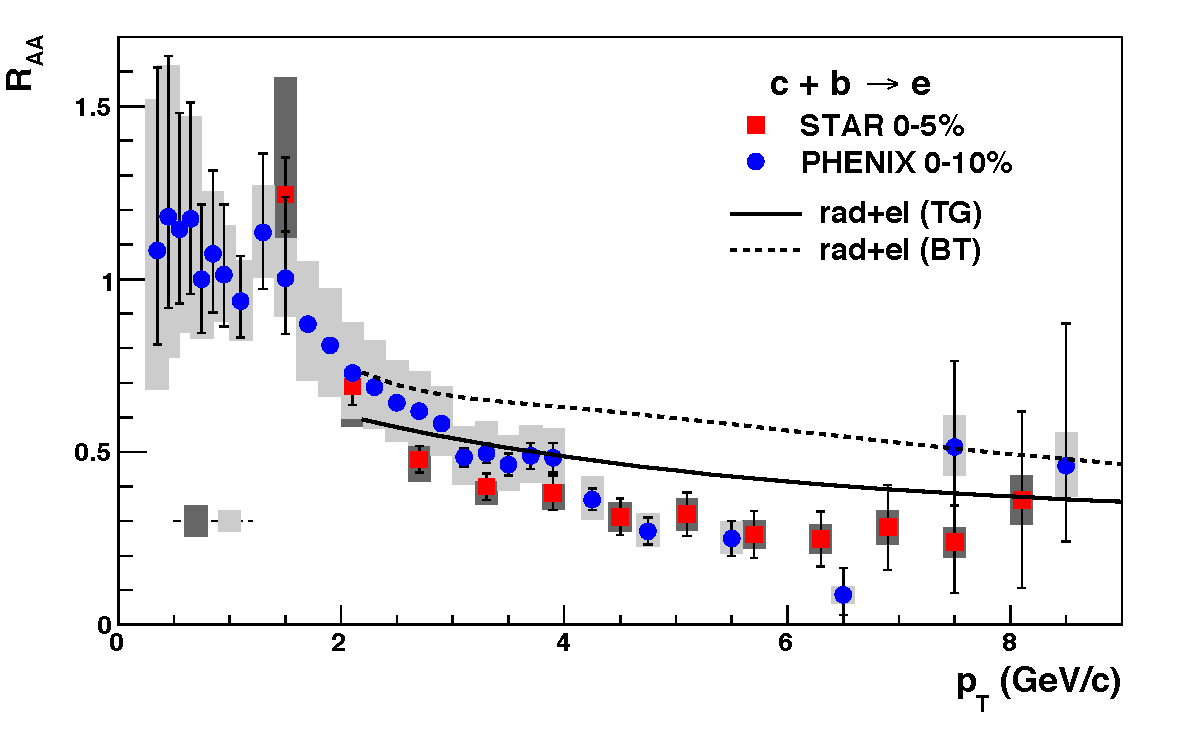
\includegraphics[width=0.35\textwidth]{fig/raa-nonphot-whdg}
%\caption{Nuclear modification factor for semi-leptonic decay electrons from $B$ and $D$ mesons, as measured by the PHENIX and STAR collaborations. Theory curves are from the ASW formalism (left plot),
%Higher Twist (center plot), and  WHDG scheme (right plot). The Higher Twist and WHDG contain both radiative and drag loss, the ASW calculations only contain radiative loss.}
%\label{non-photonic-suppression}
%\end{figure}

\begin{figure}[!htp]
   \centering
   \begin{subfigure}[b]{0.7\textwidth}
        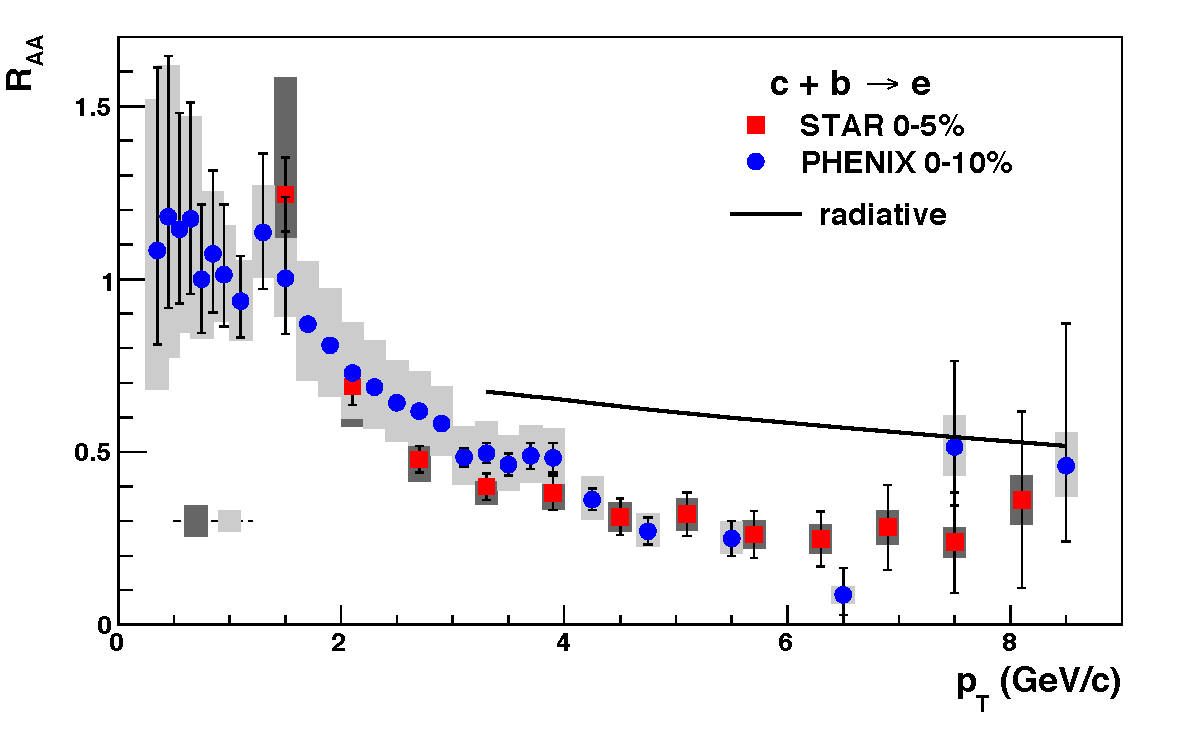
\includegraphics[width=0.90\textwidth]{fig/raa-nonphot-armesto}
       \caption{Calculations from ASW formalism\cite{Armesto:2003jh}.}
       \label{Fig:hqASW}
    \end{subfigure}
 
  \begin{subfigure}[b]{0.7\textwidth}
        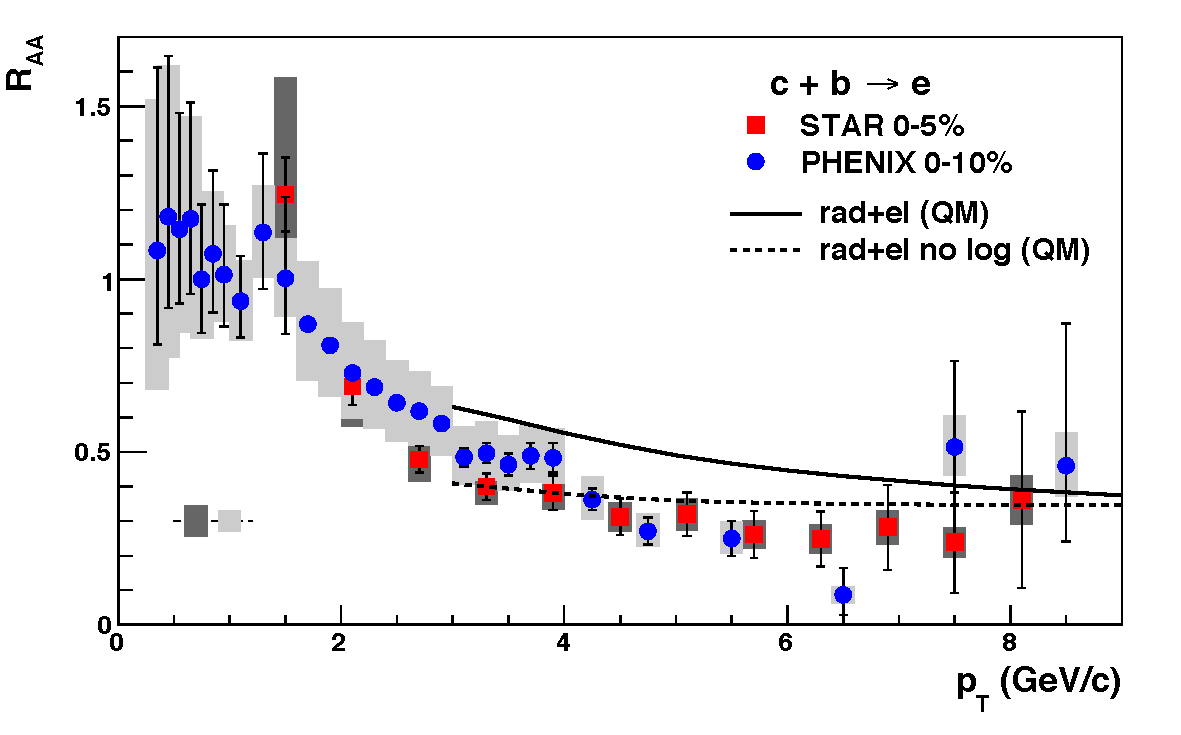
\includegraphics[width=0.90\textwidth]{fig/raa-nonphot-qin}
       \caption{Calculations from Higher Twist formalism\cite{Qin:2009gw}.}
       \label{Fig:hqHT}
    \end{subfigure}
 
  \begin{subfigure}[b]{0.7\textwidth}
        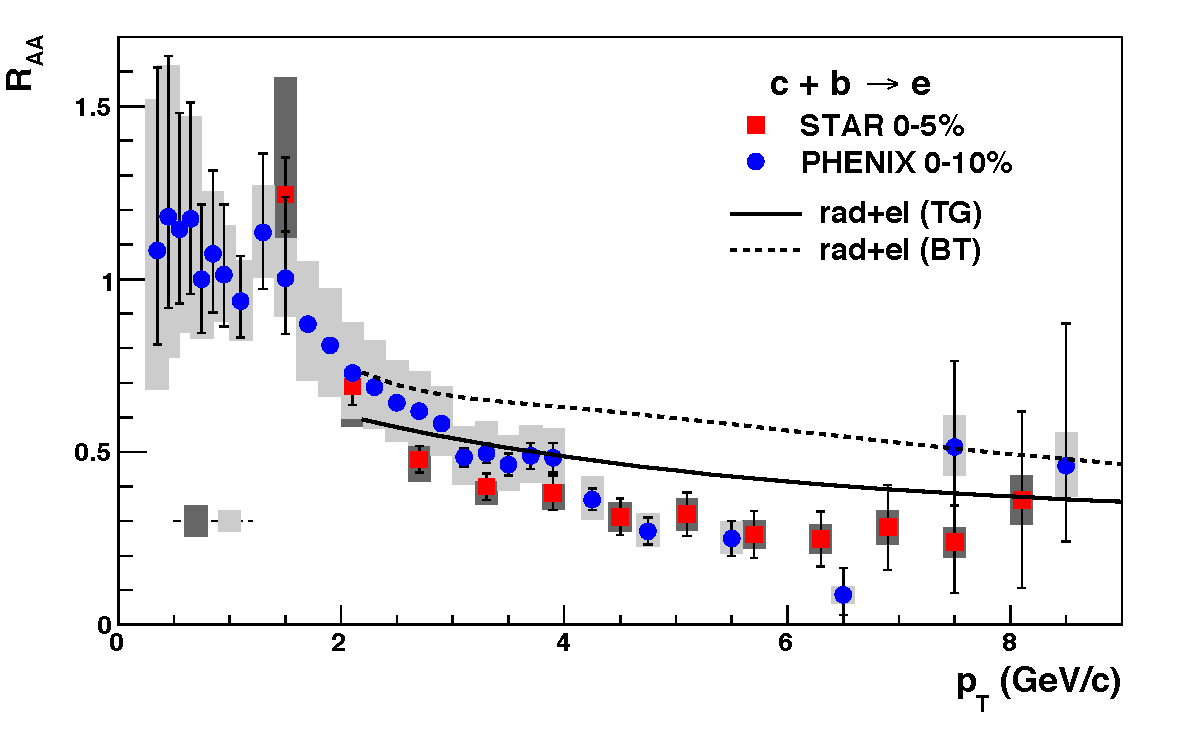
\includegraphics[width=0.90\textwidth]{fig/raa-nonphot-whdg}
       \caption{Calculations from WHDG scheme\cite{Wicks:2005gt}.}
       \label{Fig:hqWHDG}
    \end{subfigure}    
    
    \caption[Nuclear modification factor for semi-leptonic decay electrons from $B$ and $D$ mesons]{Nuclear modification factor for semi-leptonic decay electrons from $B$ and $D$ mesons, 
    as measured by the PHENIX\cite{Adare:2006nq} and STAR\cite{Abelev:2006db} collaborations compared to theory curves from various formalisms. The Higher Twist and WHDG contain both radiative and drag loss, the ASW calculations only contain radiative loss.}
\label{Fig:non-photonic-suppression}    
\end{figure}

Such measurements and associated theory calculations showed already at RHIC that heavy quarks are much more sensitive to transport coefficients such as $\hat{e}$ than the quenching of light flavors.
Statistics accumulated at the LHC allowed for much more improved comparisons by observing the $B$ and $D$ contributions separately. Indeed, at the jet energies significantly higher than the quark mass the experimental measurements of high-\pT\  $b$-quark jets show a similar suppression pattern to that of inclusive jets. In contrast, comparison of $D$-meson production and non-prompt \JPsi\ from $B$-meson decays (for $p_{T}$ up to 20 GeV/c) indicate the predicted mass hierarchy: heavy quarks loose significantly less energy as compared to the lighter flavors. The extension of these $B$/$D$ separated measurements to RHIC is a major focus of the program discussed in Section~\ref{Sec:FacilitiesFuture}.
  
\subsubsection{Outlook and Conclusions}

  Even though these studies have provided a qualitative milestone in understanding of the jet-medium interactions they call for further investigations and demand precision. As but one example, the higher statistics of future runs at the LHC are needed both to determine precisely the in-cone modifications of the energy flux associated to the jet as well as to map out the full kinematic range of the observed phenomena down to lowest jet energies. Moreover, the higher precision is needed for gamma-jet coincidences and b-jets measurements, as well as new channels of studies will become available, such as $Z$-jet coincidences.
With these measurements and their rather complete toolkit at the LHC it is compelling to perform similar measurements at the lower center-of-mass energy provided by RHIC to determine the temperature dependence of the observed phenomena. The required program, which relies on RHIC's greatly increased luminosity and upgrades to PHENIX and STAR, is discussed in detail in Section~\ref{Sec:HardProbes}. 
%Moreover, the high luminosity of the machine for the purpose of precision measurements with fully unbiased jet reconstruction can be fully explored with new instrumentation. RHIC on the contrary to LHC provides another significant advantage for the jet-medium studies by its versatile capabilities of moderating the beam energy and ion species at the heavy-ion community's demand. 

